% Created 2021-01-24 Sun 22:49
% Intended LaTeX compiler: pdflatex
\documentclass[11pt]{article}
\usepackage[utf8]{inputenc}
\usepackage[T1]{fontenc}
\usepackage{graphicx}
\usepackage{grffile}
\usepackage{longtable}
\usepackage{wrapfig}
\usepackage{rotating}
\usepackage[normalem]{ulem}
\usepackage{amsmath}
\usepackage{textcomp}
\usepackage{amssymb}
\usepackage{capt-of}
\usepackage{hyperref}
\usepackage{minted}
\hypersetup{colorlinks=true, linkcolor=black, filecolor=red, urlcolor=blue}
\usepackage[turkish]{babel}
\author{Eren Hatırnaz}
\date{12 Ocak 2020}
\title{Yazılım Gündemi - 2020/02\\\medskip
\large 6-12 Ocak 2020}
\hypersetup{
 pdfauthor={Eren Hatırnaz},
 pdftitle={Yazılım Gündemi - 2020/02},
 pdfkeywords={},
 pdfsubject={},
 pdfcreator={Emacs 27.1 (Org mode 9.3)},
 pdflang={Turkish}}
\begin{document}

\maketitle
\tableofcontents \clearpage\shorthandoff{=}

\begin{center}
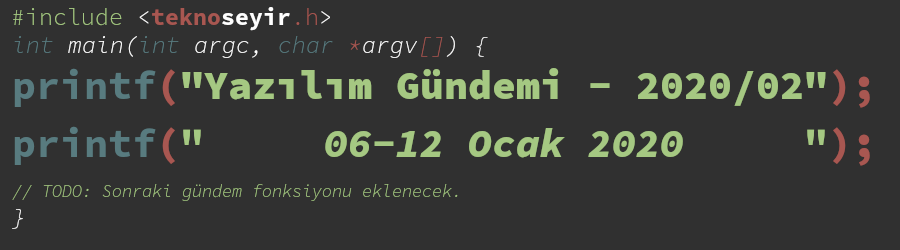
\includegraphics[width=.9\linewidth]{gorseller/yazilim-gundemi-banner.png}
\end{center}

\begin{center}
\href{../01/yazilim-gundemi-2020-01.pdf}{< Önceki Gündem} | \textbf{6-12 Ocak 2020} | \href{../03/yazilim-gundemi-2020-03.pdf}{Sonraki Gündem >}

\href{https://teknoseyir.com/blog/yazilim-gundemi-2020-02}{TeknoSeyir'de Oku}
\end{center}

\section{13 Ocak'tan itibaren Java kodları \href{https://www.alphabot.com/security/blog/2020/java/Your-Java-builds-might-break-starting-January-13th.html?utm\_name=iossmf}{derlemede sorun yaşayabilirsiniz}}
\label{sec:org18e2733}
\begin{center}

\includegraphics[height=2cm]{gorseller/java-https.png}
\end{center}

Daha önce de sıkça bahsettiğim gibi günümüzün yazılım geliştirme süreçlerinde
üçüncü parti kütüphaneler ve araçlar artık neredeyse olmazsa olmazlardan biri.
Kendimiz yapsak farklı sorunlarla karşılaşacağımız ya da vaktimizi alacak
birçok ihtiyacımızı bu üçüncü parti kütüphaneler ve araçlarla gideriyoruz fakat
beraberinde getirdiği riskler de yok değil. İşte bu risklerden biri olan
MITM(Man-in-the-middle) saldırılarını önlemek için Java ekosistemindeki üçüncü
parti kütüphane depoları (artifact repository) sadece HTTPS bağlantılarına izin
verecekler. Tabii ki bu kararı yeni almadılar, önceden duyurmuşlardı fakat yine
de hatırlatmak için gündeme almak istedim. Popüler bazı depoların HTTP
desteklerini sonlandıracakları tarihler bu şekilde:

\begin{itemize}
\item JCenter(JFrog Bintray) | \url{http://jcenter.bintray.com} : \textbf{13 Ocak 2020}.
\href{https://jfrog.com/blog/secure-jcenter-with-https/}{Duyuru yazısı}
\item Maven Central | \url{http://repo1.maven.org}, \url{http://repo.maven.apache.org}: \textbf{15
Ocak 2020}. \href{https://central.sonatype.org/articles/2019/Apr/30/http-access-to-repo1mavenorg-and-repomavenapacheorg-is-being-deprecated/}{Duyuru yazısı}
\item Spring (Pivotal) | \url{http://repo.spring.io}: \textbf{15 Ocak 2020}. \href{https://spring.io/blog/2019/09/16/goodbye-http-repo-spring-use-https}{Duyuru yazısı}
\item Gradle | \url{http://repo.gradle.org}: \textbf{15 Ocak 2020}. \href{https://blog.gradle.org/decommissioning-http}{Duyuru yazısı}
\end{itemize}

Bu değişiklikten etkilenmemek için ilgili depoların yayınladıkları duyuru
yazılarındaki yönergeleri uygulamalısınız.

Elbette üçüncü parti kütüphaneler ile ilgili tek sorun MITM saldırıları değil.
Projeye eklediğimiz kütüphaneyle birlikte o kütüphanenin varsa güvenlik
açıklarını da projeye ekliyoruz. \href{../../2019/01/yazilim-gundemi-01.pdf}{İlk yazılım gündemi yazısı}ndan beri sürekli
çeşitli kütüphanelerdeki açıkların etkileriyle ilgili konuları işliyorum.
Hacker'lar artık son kullanıcı yerine direkt bizim kodlarımızı kullanarak
içeriye girmeye çalışıyorlar, bu alanı keşfettiler. Dolayısıyla projemize
bağımlılık olarak bir kütüphane eklerken, körü körüne eklemek yerine en azından
kodlarına şöyle bir göz gezdirmekte fayda var.
\section{TypeScript 3.8 Beta \href{https://devblogs.microsoft.com/typescript/announcing-typescript-3-8-beta}{duyuruldu}}
\label{sec:org8171fc7}
Microsoft tarafından geliştirilen ve gittikçe popülaritesi artan dillerden
TypeScript, 3.8 Beta sürümünü bu hafta içerisinde yayınladı. Bu sürüm ile
birlikte gelen bir özelliği inceleyelim:
\subsection{Private Fields}
\label{sec:org84781f3}
ECMAScript'de \href{https://tc39.es/process-document/}{stage-3 aşaması}na geçen \href{https://github.com/tc39/proposal-class-fields/}{class fields} özelliğinin \href{https://github.com/tc39/proposal-class-fields/\#private-fields}{bir parçası}
aslında bu özellik. Diğer dillerde görmeye alışık olduğumuz class'a ait bir
özelliğin dışarıdan erişilemez olmasını sağlıyor. Örneğin:
\begin{minted}[breaklines=true,breakanywhere=true,frame=lines, linenos, label=TypeScript, labelposition=topline]{typescript}
class Kisi {
    #isim: string

    constructor(isim: string) {
        this.#isim = isim;
    }

    selamla() {
        console.log("Selam, benim adım ${this.#isim}!");
    }
}

let eren = new Kisi("Eren Hatırnaz");

eren.#isim
\end{minted}
Artık böyle bir kod yazmak mümkün olacak ve son satırdaki gibi sınıfın dışından
bir erişim yapılmaya çalışılırsa şu hata alınacak:
\begin{quote}
Property '\#isim' is not accessible outside class 'Kisi' because it has a
private identifier.
\end{quote}
Fakat bu özelliği kullanmak için şunları unutmamalıyız:
\begin{itemize}
\item Private field'lar \texttt{\#} karakteri ile başlamalıdır ve sınıf içerisinde aynı
şekilde çağırılmalıdır.
\item Her private field sadece kendi sınıfı içerisinde private durumundadır.
\item TypeScript'deki diğer \texttt{public} ve \texttt{private} gibi anahtar kelimeler bu
özellikle birlikte kullanılamaz.
\end{itemize}
Bazı maddeler tam anlaşılmamış olabilir fakat örneklerle birlikte açıklamak
yazıyı biraz uzatacağı için bu özellikle ilgili arkadaşları konu bağlığına
eklediğim bağlantıya tıklayamaya davet ediyorum.
\section{WebAssembly kullanan sitelerin birçoğu kötü amaçlı kullanıyor}
\label{sec:org3c1ec1a}
Geçtiğimiz haftalarda W3C tarafından bir web standardı olarak kabul edilen
WebAssembly programlama dili performanslı olmasıyla öne çıktığı için kötü
amaçlı kişilerin de gözünden kaçamamış maalesef. Geçtiğimiz sene yayınlanan \href{https://www.sec.cs.tu-bs.de/pubs/2019a-dimva.pdf}{bir
akademik çalışma} ortaya koydu ki Alexa'nın popüler ilk 1 milyon web sitesi
içerisindeki sitelerden WebAssembly kullananların birçoğu bunu kötü amaçlarına
alet ediyorlarmış.

\begin{center}
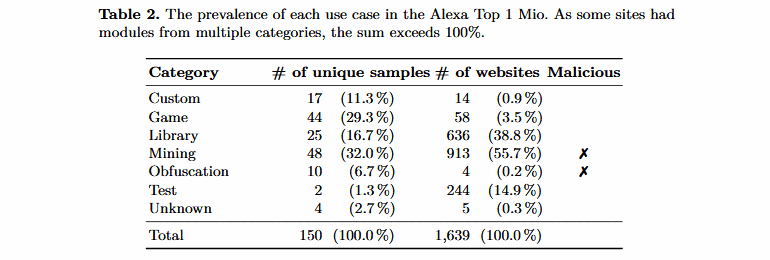
\includegraphics[width=.9\linewidth]{gorseller/webassembly-kotu-amaclar.png}
\end{center}

Araştırmacılar Alexa'nın ilk 1 milyon web sitesinden rastgele seçilmiş 3
sayfayı seçeyerek bu sayfada WebAssembly kodu olup olmadığını analiz etmişler
ve toplam 1.639 web sitesinin WebAssembly kodu içerdiğini tespit etmişler.
Bunlardan bazıları diğer birçok site tarafından kullanılan kütüphaneler fakat
araştırmacılar diğer yaygın olmayan kodları incelediğinde bazılarının kripto
para madenciliği amacıyla yazıldığını fark etmişler. Dil hem performanslı hem
de tarayıcıda çalışınca işte fırsatı kaçırmamışlar.

Bazı web sayfalarının ise obfuscate yöntemleri kullanarak WebAssembly
kodlarının içeriğini gizlediğini fark etmişler. Araştırmacılar bu kategori için
de "malicious" diye tanımlamışlar ama ben tam öyle düşünmüyorum. Her ne kadar
kodlarını saklamalarında biraz şüphe olsa da insanlar kodlarını saklamayı
seçebilirler, bu illaki kötü amaçlı olacaklarını göstermez.

İşte siber güvenlik alanında çalışacaklar için yeni bir alt alan daha. Web
standardı olarak kabul edilmesiyle birlikte bu tarz amaçlar için kullanan
kişilerin de artacağını düşünüyorum. Siber güvenlik alanıyla ilgili
arkadaşların araştırmalarını tavsiye ederim.
\section{Yaklaşan Etkinlikler}
\label{sec:org89ff0e4}
\begin{longtable}{|p{8cm}|l|l|}
\hline
Etkinlik İsmi & Yeri & Tarihi\\
\hline
\endfirsthead
\multicolumn{3}{l}{Önceki sayfadan devam ediyor} \\
\hline

Etkinlik İsmi & Yeri & Tarihi \\

\hline
\endhead
\hline\multicolumn{3}{r}{Devamı sonraki sayfada} \\
\endfoot
\endlastfoot
\hline
\href{https://www.meetup.com/Cozumpark/events/267512181/}{Bulutun Geleceği, Hibrit Bulut \{Webcast\}} & Online & 14 Ocak 10:00\\
\href{https://www.meetup.com/NS-Ankara/events/267855245/}{NS Ankara Ocak Ayı 1.Buluşması} & Ankara & 14 Ocak 19:00\\
\href{https://www.eventbrite.com/e/trai-meet-up-30-biyometrik-guvenlik-ve-yapay-zeka-tickets-88912765475}{TRAI Meet-up 30 - Biyometrik Güvenlik ve Yapay Zeka} & İstanbul & 15 Ocak 18:00\\
\href{https://www.eventbrite.com/e/devc-istanbul-semi-ideathon-tickets-88393923605}{DevC İstanbul Semi Ideathon} & İstanbul & 18 Ocak 07:00\\
\href{https://www.meetup.com/GDGAnkara/events/267812348/}{Women Techmakers Series} & Ankara & 18 Ocak 11:00\\
\href{https://www.eventbrite.com/e/mobile-game-meetup-tickets-88795231929}{Mobile Game Meetup} & İstanbul & 18 Ocak 13:00\\
\href{https://www.eventbrite.com/e/game-meetup1-tickets-88215020501}{Game Meetup'1} & İstanbul & 20 Ocak 11:00\\
\href{https://www.meetup.com/Microsoft-Giri\%25C5\%259Fimcilik-Bulu\%25C5\%259Fmalar\%25C4\%25B1/events/267510267/}{F2P Mobil Oyunlar için Metrikler ve Analiz Rehberi} & Ankara & 21 Ocak 19:00\\
\href{https://www.meetup.com/IzmirGophers/events/267488435/}{Test Driven Development ve Clean Architecture} & İzmir & 21 Ocak 19:00\\
\href{https://www.meetup.com/PostgreSQL-TR/events/267534661/}{PostgreSQL Konuşmaları: Pgbadger ile Log Analizi ve Performans İzleme} & Ankara & 21 Ocak 19:00\\
\href{https://kommunity.com/devops-turkiye/events/infrastructure-as-software}{Infrastructure as Software} & İstanbul & 23 Ocak 18:30\\
\href{https://kommunity.com/devnot-yazilimci-bulusmalari/events/promethues-ve-grafana-ile-metrik-olusturma-ve-goruntuleme}{Promethues ve Grafana ile Metrik Oluşturma ve Görüntüleme} & İstanbul & 24 Ocak 19:00\\
\hline
\end{longtable}
\section{Diğer Haberler}
\label{sec:org77b434b}
\begin{itemize}
\item D programlama dilinin 2.090.0 \href{https://dlang.org/changelog/2.090.0.html}{sürümü duyuruldu}.
\item Kubernetes için yeni \href{https://grafana.com/blog/2020/01/09/introducing-tanka-our-way-of-deploying-to-kubernetes/}{bir araç tanıtıltı}: \href{https://github.com/grafana/tanka}{Grafana Tanka}.
\item Idris programlama dilinin geliştiricisi \href{https://www.type-driven.org.uk/edwinb/linearity-and-erasure-in-idris-2.html}{Idris 2 üzerinde çalışıyormuş}.
\item Testlerde kullanmak için sahte API'ler oluşturmaya yarayan \href{https://nehalist.io/mocking-hans/}{yeni bir araç
tanıtıldı}: \href{https://github.com/loremipsum/mocking-hans}{Mocking Hans}.
\item Python için HTTP istemcisi olan \href{https://github.com/encode/httpx}{HTTPX} kütüphanesinin 0.11.0 \href{https://github.com/encode/httpx/releases/tag/0.11.0}{sürümü
yayınlandı}.
\item \href{https://github.com/sagiegurari/duckscript}{DuckScript} dilinin 0.1.5 \href{https://github.com/sagiegurari/duckscript/releases/tag/0.1.5}{sürümü yayınlandı}.
\item \href{https://github.com/dafer45/TBTK}{TBTK} kütüphanesinin \href{https://github.com/dafer45/TBTK/releases/tag/v2.0.0}{v2.0.0 sürümü yayınlandı}.
\item \href{https://github.com/dtolnay/cxx}{CXX} kütüphanesinin ilk versiyonu \href{https://github.com/dtolnay/cxx/releases/tag/0.1.0}{0.1.0 yayınlandı}.
\item Terminal ekranında grafiksel kullanıcı arayüzleri oluşturmaya yarayan C\#
kütüphanesi \href{https://github.com/goblinfactory/konsole/}{Konsole}'nin 5.4.2 \href{https://github.com/goblinfactory/konsole/releases/tag/5.4.2}{sürümü duyuruldu}.
\end{itemize}
\section{Lisans}
\label{sec:org14cdb47}
\begin{center}
\begin{center}

\includegraphics[height=1.5cm]{../../../img/CC_BY-NC-SA_4.0.png}
\end{center}

\href{yazilim-gundemi-2020-02.pdf}{Yazılım Gündemi - 2020/02} yazısı \href{https://erenhatirnaz.github.io}{Eren Hatırnaz} tarafından \href{http://creativecommons.org/licenses/by-nc-sa/4.0/}{Creative Commons
Atıf-GayriTicari-AynıLisanslaPaylaş 4.0 Uluslararası Lisansı} (CC BY-NC-SA 4.0)
ile lisanslanmıştır.
\end{center}
\end{document}
